\documentclass[12pt]{aastex62}
\usepackage[utf8]{inputenc}
\usepackage[english]{babel}
 
%\usepackage{multicol}
\usepackage{amsmath}
\usepackage{amssymb}
\usepackage{amsfonts}
\makeatletter
\def\amsbb{\use@mathgroup \M@U \symAMSb}
\makeatother
\usepackage{bbold}
\usepackage{amsthm}
\usepackage{tabularx}
\usepackage[]{hyperref}
%\usepackage{graphicx}
%\usepackage{subcaption}
%\graphicspath{ {Figures/} }


\topmargin 0.0cm
\oddsidemargin 0.2cm
\textwidth 16cm 
\textheight 21cm
\footskip 1.0cm

\newtheorem{prop}{Proposition}
\theoremstyle{definition}
\newtheorem{defn}{Definition}

\DeclareMathAlphabet{\pazocal}{OMS}{zplm}{m}{n}
\DeclareMathOperator*{\argmin}{arg\,min}


\begin{document}
\title{A Framework for Telescope Schedulers: With Applications to the Large Synoptic Survey Telescope}
\author{Elahesadat Naghib, Peter Yoachim, Robert J. Vanderbei, Andrew J. Connolly}

%\affil[a]{Princeton University}
%\affil[b]{Princeton University}
%s\affil[c]{University of Washington}
%\maketitle
%\begin{multicols}{2}

\begin{center}
\textbf{Key terms and notations}\
\noindent\rule{\textwidth}{0.4pt}
\end{center}

\begin{table}[h]
\begin{tabularx}{\textwidth}{l  X }
fields & fixed partitions of the sky that can be covered in a single visit, \\
$N_{f}$ & total number of the fields,\\
$t$& Greenwich Mean Time, in Modified Julian Date,\\ 
$\tau_s(t)$ ($\tau_e(t)$)& beginning (end) of the night that $t$ lies in,\\
$\tau_{rise\text{(}set\text{)}}(i,f,t)$ & rising (setting) time of field-filter $(i,f)$ above (below) the acceptable airmass horizon at current night,\\
$\tau_n(i,f,t)$& time of the last visit of field-filter $(i,f)$ before $\tau_s(t)$,\\
$id(t)$ & ID number of the field that is visited at $t$,\\
$ft(t)$& camera's filter at $t$,\\
$n(i,f,t)$ & total number of the visits of field-filter $(i,f)$ before $t$,\\
$slew(i,j)$& slew time from field $i$ to field $j$ in seconds,\\
$settling(i,j)$& mechanical settling time after slewing from field $i$ to field $j$,\\
$\Delta t_{f}$& time needed to change filter, a constant value about 2 minutes,\\
$t_{dome}(i)$& time needed to move the dome to make field $i$ visible to the telescope,\\
$ha(i,t)$ & hour angle of the center of field $i$ at $t$ in hours, $-12 \leq ha(i,t) \leq 12$,\\
$am(i,t)$ & airmass of the center of field $i$ at $t$,\\
$br(i,t)$ & brightness of the sky at the center of field $i$ at $t$,\\
$\sigma(i,t)$ & seeing of the sky at the center of field $i$ at $t$,\\
$K(i,f, t)$ & atmospheric extinction coefficient\\
$W_1, W_2$ & given constant time window within which a revisit is valid, \\
$I_{survey}$ & set of all fields in $survey \in \{WFD,DD,NES,GP,SCP\}$ ,\\
\end{tabularx}
\end{table}
\noindent\rule{\textwidth}{0.4pt}\\
\newpage

\begin{abstract}

Feature-Based telescope scheduler is an automated, proposal-free decision making algorithm that offers \textit{controllability} of the behavior, \textit{adjustability} of the mission, and quick \textit{recoverability} from interruptions for large ground-based telescopes. It is easy to understand, implement and troubleshoot because of its coherent mathematical representation. Accordingly it can be modified by the astronomy community for context-dependent adjustments. This paper presents a raw version of the Feature-Based scheduler, with minimal manual tailoring, to demonstrate its potential and flexibility as a foundation for large ground-based telescope schedulers that can later be adjusted based on the specifications of each instrument. In addition, an improved version of the Feature-Based scheduler for LSST is briefly introduced and compared to previous LSST scheduler simulations.
\end{abstract}

\section{Introduction}

The Large Synoptic Survey telescope (LSST), the top national ground-based telescope of the 2010 Decadal Review, with the largest digital camera that has ever been built for astronomy, offers an optical throughput of more than $200~m^2 deg^2$ which is 50 times greater than the best current value \citep{tyson2002large}. Scientific investigations with LSST range from the solar system objects to the edge of the optical universe. 

Even with the powerful engine that enables this telescope to slew fast, satisfying all of the science-driven desirables and constraints is a challenging problem. Specifically, the LSST's science-driven mission (explained in \citep{ivezic2008large}) is highly constrained and contains competing objectives that are vastly different in nature, due to the different nature of the scientific expectations. In this paper, we propose a framework to formulate the problem of scheduling for large ground-based telescopes such as LSST then derive a scheduler based on the proposed model.

First generation schedulers for astronomical purposes were developed for space missions to automate their operation due to their inaccessibility and more importantly, to optimize their scientific productivity. ROSAT mission's scheduler in 1990 \citep{nowakovski1999using},  Spike \citep{johnston1994spike}, Hubble Telescope's scheduler in 1994, and HSTS \citep{muscettola1995automating} in 1995 are amongst pioneering developments on algorithmic scheduling of observations in the space missions. 

Despite the similarity of the ultimate goal in the missions of both space telescopes and ground-based telescopes, determining factors for the purpose of scheduling are fundamentally different. While space-based telescopes are required to respect kinematical and dynamical constraints, earth's atmosphere is the main challenge in the scheduling of ground-based telescopes. The former is predictable and efficiently computable, while the later involves both inherent uncertainties, and uncertainties due to the computational limitations. 

Earlier systematic approaches to the scheduling of ground-based telescopes are heavily based on hand-crafted observation proposals that are generally tested only for feasibility, but not necessarily for optimality. For instance,  Keck Telescope, 1993 \citep{nelson1985design} is run 100\% based on proposals, and Hobby-Eberly Telescope 1997 \citep{shetrone2007ten} has a semi-manual scheduling scheme. 

Later, appearance of more expensive ground-based instruments with complex missions made it impossible to rely on hand-crafted proposals solely. Need for more efficient use of the instrument's time lead to the development of decision making algorithms for accessible facilities as well, and mainly to optimize their science output. For instance, scheduler of the Liverpool robotic telescope was designed in 1997 to automate and optimize the procedure of time allocation to the chunks of scripted schedules. Time allocation strategy was preferred to the scheduling at the single visit level which is referred to as optimum scheduling by the authors of \citep{steele1997control}. The reason for choosing the time allocation scheme instead of optimum scheduling is stated to be the lack of recoverability of the latter choice in case of an interruption, because it potentially leads to excessive computational cost to reevaluate the sequence, one-by-one once it is interrupted. In this paper, we show that scheduling in the single visit level can be quickly recoverable in a memoryless framework, thus the optimality can be preserved. Another example is the Las Cumbres Observatory Global Telescope Network (LCOGT) with one of the most advanced telescope scheduling algorithms \citep{Boroson14, Saunders14}. LCOGT uses an integer linear programming (ILP) model, solved with the Gurobi algorithm \citep{gurobi}, to optimize the scheduling of observations over a global network of telescopes \citep{Lampoudi15}. Due to the success of this approach the Zwicky Transient Facility at Palomar Observatory \citep{Bellm14} has also adopted a ILP scheduler\footnote{\url{https://github.com/ZwickyTransientFacility/ztf_sim}}. The ILP model performs well for observatories where slew overheads are small compared to exposure execution time. LCOGT is able to schedule observations in long contiguous blocks. In contrast, the LSST plans to have observations of order 30 seconds with slew times up to 2 minutes, hence it requires a scheduling algorithm that can explicitly minimize the slew times between successive observations. One could use the ILP approach to schedule large prescript blocks of observations for the LSST. The blocks could be set to follow a path that only includes short slews (this is close to the strategy taken in the scheduler developed by D. Rothchild et al. (2018, in preparation). The disadvantage of this approach and any other prescript schedule is principally the lack of recoverability from unpredictable conditions, for instance inability to dodge the clouds.

Still, in spite of the reliability of the fully automatic scheduling technologies, there are modern, expensive telescopes such as SALT, 2005 \citep{brink2008salt}, and ALMA 2013 \citep{wootten2003atacama} that are run based only on traditional hand-crafted proposals. ALMA in particular, requires a highly regulated structure for proposals that potentially leads to suboptimality as discussed in \citep{alexander2017enabling}, where the authors suggest a number of corrections for the scheduling regulations to provide adaptivity to time-sensitive observations. However, even with occasional corrections, a verbal policy does not provide verifiable adjustability to the change of mission, as the operation of the telescope reveals newfound scientific desirables. It seems that refusing to adopt the progressive technology of fully automated scheduling for modern instruments is mainly due to the rooted notion of the observation proposals that perfectly served the scheduling of smaller, and slower instruments in the past. This also could be a result of astronomer's lack of trust toward the performance of the decision making machines in every levels of the scheduling. The LSST community, however, in addition to a proposal-based scheduler, introduced in \citep{delgado2016lsst}, have been supporting the design and implementation of proposal-free decision machines, such as Feature-Based scheduler, first introduced in \citep{naghib2016feature}, as well as a variant of the fast marching army cadence by D. Rothchild et al. (2018, in preparation) that explore the possibility of a new generation of the schedulers for fast, expensive, and multi-mission instruments. The LSST in particular, will be able to make 1000 observations on a clear night, for which the scheme of manual scheduling is completely outdated and inefficient, because with the slew-efficiency and the order of visits becomes a determining factor, as opposed to slower, or single mission telescopes that are only required to visit a limited number of the prescript objects, usually independent of the slew trajectory and efficiency.



In Section~\ref{sec_SM}, first we explain the choice of Markovian framework for Feature-Based scheduler, and in Sections~\ref{sec_Markov} and~\ref{sec_Markov_approx} we provide the mathematical details of the scheduler model in that framework. Section~\ref{sec_opt} presents two approaches for the optimization of the model's parameters. Sections~\ref{sec_lsst_problem} and~\ref{sec_lsst_opt} demonstrate the application of the Feature-Based scheduler on LSST which is then followed by a comparison between an improved version of the Feature-Based scheduler and LSST's current official scheduler in Section~\ref{sec_comp}. Finally, Section~\ref{sec_conclusion} presents our concluding remarks.



\section{Scheduling framework}\label{sec_SM}

To run a multi-mission, highly constrained telescope such as LSST, the scheduler has to offer \textit{controllability}, \textit{adjustability}, and \textit{recoverability}, as explained in the following.

\begin{itemize}
\item \textbf{Controllability}: The high-level mission objectives have to show sufficient variabilities with the variation of the model parameters. Otherwise, either the choice of the input  information is irrelevant to the mission objectives, or the structure of the scheduler is degenerate. High-level objective functions of a controllable scheduler have meaningful correlations with each of the model parameters. This property is necessary for the scheduler to be optimizable by the optimal choice of the model parameters.

\item \textbf{Adjustability}: For a complex, multi-objective mission it is common that the high-level objectives are required to be adjusted in the middle of the operational period. Adjustments take place according to a new set of scientific desirables, or based on a feedback provided by the study of the system's performance. Regardless of the reason for the adjustments, a scheduler must offer a systematic flexibility to be adjusted with a reasonable computational cost, and preferably no expert intervention. Hand-tuned scheduling strategies and verbal policies for instance, are not fully adjustable.

\item \textbf{Recoverability}: The presence of unpredictable factors in the operation of ground-based telescopes are due to the natural stochastic processes (such as the weather), and complexity of the mechanical facility that brings randomness to the decision procedure. Unscheduled downtimes and filter breakdowns are examples of the many unpredictable survey interruptions. On the other hand, there are inherently predictable interruptions, such as maintenance downtimes, and cable winding that also, due to the complexity of the mechanical system, are not computationally affordable and/or valuable to keep track of. Therefore, they are considered as stochastic variables as well. Given all the stochastic factors, a scheduler is required to be able to quickly output an alternative decision, once a previously unpredictable variable took a value, as well as occurrence of an interruption, for which the scheduler is expected to return to its normal behavior, as fast as possible. A pre-calculated sequence of decisions for instance, lacks the recoverability attribute. Also, strategies with heavy look-back or look-ahead are not fast recoverables. 
\end{itemize}

The Feature-Based scheduler is designed based on a Markovian model in which the flow of the input information, the decision procedure and it's relationship to the mission's objective is coherently expressed, therefore, controllability of the scheduler is well-defined and observable as presented in Section~\ref{sec_sim_cont}. And it is adjustable, because of the Markovian structure that offers an explicit derivation of the design elements from high-level objectives, and finally is swiftly recoverable due to the inherent memorylessness of the Markovian decision process that for a decision at any time, only requires the current state of the system.

\subsection{Markovian representation}\label{sec_Markov}

\begin{defn}
Let $X_{(.)}$ be a stochastic process for which $X_i$ represents the state of the system at $t_i$, and $\pazocal{S}$ be the set of all possible states that the system can take. Let $\mathbb{P}(X_i)$, be the probability distribution of $X_i$ on $\pazocal{S}$, then $X(.)$ is a Markovian process, if and only if, it satisfies the following \textit{memorylessness} property,
\begin{equation*}
\forall i ~~~~~~~\mathbb{P}(X_{{i+1}} | X_{i}) = \mathbb{P}(X_{{i+1}} | X_{i}, X_{{i-1}},\dots, X_{0}),
\end{equation*}
where $\mathbb{P}(X_{{i+1}} | X_{i})$ is the conditional probability distribution of the system's state at $t_{i+1}$ given it's state at $t_i$, and $\mathbb{P}(X_{{i+1}} | X_{i}, X_{{i-1}},\dots, X_{0})$ is the conditional probability distribution of the system's state at $t_{i+1}$, given all of the states that the system has been in until $t_i$.
\end{defn}

Memorylessness property asserts that the system's next state only depends on its current state and is independent of its earlier history. This property, is in fact, the main reason for choosing a Markovian framework for the scheduler. Accordingly, in the modeling level it requires a state description such that the behavior of the system can be determined by the current state of the system. And consequently, in the scheduling level, a decision can be made based only on the current state of the system.

\begin{defn}
Let $<\pazocal{S},\pazocal{A}, P_a(.,.), R_a(.,.), \gamma>$, be a \textit{Markovian Decision Process (MDP)}, where $\pazocal{A}$ is the set of actions, and $P_a(x, y)$ transition probability from state $x$ to $y$ which is equal to $\mathbb{P}(X_{i+1}=y | X_i=x, a)$, conditional probability of transition from state $x$ to state $y$ given action $a \in  \pazocal{A}$. Similarly the transition reward is denoted by $R_a(x,y)$, and $\gamma \in (0,1]$ is the discount factor.
\end{defn}

\begin{defn}
Action $a_{i} \in \pazocal{A}$ is \textit{admissible} for $<\pazocal{S},\pazocal{A}, P_a(.,.), R_a(.,.), \gamma>$, if it is,
\begin{enumerate}
\item feasible: It is possible to be taken at $t_i$,
\item progressively measurable: only dependent on the current state of the system $X_i$.
\end{enumerate}
\end{defn}

To control the system is to take an action at all decision steps $t_i$. For a Markovian control, the actions are required to be dependent only on the current state to preserve the memorylessness property of the closed-loop system, that's why we require the action to be progressively measurable.

Notice that the decision steps $\{ t_i: 0 \leq i \leq N, t^N  =T\}$, from $t_0$, start of the process, to $T$, time horizon of the process, are not necessarily uniformly spaced, and are determined by the time that each transition takes. 

\begin{defn}
A \textit{deterministic policy} $\pi : \pazocal{S} \rightarrow \pazocal{A}_i$, is a mapping from $\pazocal{S}$ to the set of all admissible actions at $t_i$, denoted by $\pazocal{A}_i$. 
\end{defn}

A policy provides a time invariant control law that for all possible $x_i \in \pazocal{S}$ suggests an admissible action for transition to the next state, which automates the control of the system.

\begin{defn}
\textit{A deterministic optimal policy} $\pi$ is a solution to the following optimization problem,
\begin{equation}\label{equ_opt1}
\begin{aligned}
& \underset{\pi}{\text{maximize}}
& & E_{\pi}[\sum_{i = 0}^N \gamma^i R_{\pi(X_{i-1})}(X_{i-1}, X_{i}) | x_0],
\end{aligned}
\end{equation}
where $x_0$ is a given initial state.
\end{defn}

In other words, a deterministic optimal policy maximizes the expected discounted sum of the rewards. By discounting the later rewards versus earlier rewards through $\gamma$, we tune the priority of the overall gain versus instant gains.

\begin{prop} \label{prop_main}
For the Markove decision process of $<\pazocal{S},\pazocal{A}, P_a(.,.), R_a(.,.), \gamma>$, there exists a deterministic optimal policy, and it can be written as follows, 
\begin{equation}\label{equ_opt_pol}
\pi^*= \argmin_{a_{i} \in \pazocal{A}_i} E[\Phi(X_{{i+1}}) | a_{i}],
\end{equation}

where $\Phi: \pazocal{S} \rightarrow \rm I\!R$ is a function.
\end{prop}

\begin{proof}
Consider a function $C_{\pi}: \pazocal{S} \rightarrow \rm I\!R$, defined as follows,

\begin{equation*}
\begin{aligned}
C_{\pi}(x_{i}) &= -E_{\pi}[ \sum_{i\leq j}^N \gamma^{i - j} R_{\pi(X_j)}(X_{j}, X_{{j+1}}) |x_{i}]\\
& = - E_{\pi}[R_{\pi(x_i)}(x_{i}, X_{{i+1}}) | x_{i}] - \gamma E_{\pi}[ \sum_{ i+1 \leq j}^N \gamma^{j-(i+1)} R_{\pi(X_j)}(X_{j}, X_{j+1}) | x_{i}].\\
\end{aligned}
\end{equation*}

Then by applying the the law of total expectation on the second term,

\begin{equation*}
\begin{aligned}
C_{\pi}(x_{{i}}) &= - E_{\pi}[R_{\pi(x_i)}(x_{i}, X_{{i+1}}) | x_{i}] - \gamma E_{\pi}[ E_{\pi}[ \sum_{ i+1 \leq j}^N R_{\pi(X_j)}(X_{j}, X_{{j+1}}) |X_{{i+1}}]| x_{i}]\\
&=  - E_{\pi}[R_{\pi(x_i)}(x_{i}, X_{{i+1}}) | x_{i}] - \gamma E_{\pi}[ C_{\pi}({X_{{i+1}}})| x_{i}],
\end{aligned}
\end{equation*}
and by assuming a finite state space,
\begin{equation*}
C_{\pi}(x_{{i}}) =  - E_{\pi}[R_{\pi(x_i)}(x_{i}, X_{{i+1}}) | x_{i}]  - \gamma \sum_{x_{i+1} \in \pazocal{S}} \mathbb P(x_{i+1}|\pi(x_i), x_{i}, x_{i-1},\dots, x_{0}) C_{\pi}({x_{{i+1}}}).\\
\end{equation*}

Then by the Markov property,

\begin{equation*}
\begin{aligned}
C_{\pi}(x_{i}) &=  - E_{\pi}[R_{\pi(x_i)}(x_{i}, X_{{i+1}}) | x_{i}] - \gamma \sum_{x_{i+1} \in \pazocal{S}} P_{\pi(x_{i})}(x_{i},x_{i+1}) C_{\pi}({x_{{i+1}}}),\\
\end{aligned}
\end{equation*}
where, $P_{\pi(x_{i})}(x_{i},x_{i+1}) $ is the transition probability from $x_i$ to $x_{i+1}$ under the action of $\pi(x_i)$. 

Now, let $C^*(x_{i}) = \min_{\pi} C_{\pi}(x_{{i}})$ then,

\begin{equation}\label{equ_proof1}
\begin{aligned}
C^{*}(x_{{i}}) &=  ~~~~~~~ \min_{\pi}(- E_{\pi}[R_{\pi(x_i)}(x_{i}, X_{{i+1}}) | x_{i}] - \gamma \sum_{x_{i+1} \in \pazocal{S}} P_{\pi(x_{i})}(x_{i},x_{i+1}) C_{\pi}({x_{{i+1}}}))\\
& =  \min_{\{\pi(x_{i}), \pi(x_{{i+1}}),\dots \}}(- E_{\pi}[R_{\pi(x_i)}(x_{i}, X_{{i+1}}) | x_{i}] - \gamma \sum_{x_{i+1} \in \pazocal{S}} P_{\pi(x_{i})}(x_{i},x_{i+1}) C_{\pi}({x_{{i+1}}}))\\
& = ~~~~~~~ \min_{\pi(x_{i})} (- E_{\pi}[R_{\pi(x_i)}(x_{i}, X_{{i+1}}) | x_{i}] - \min_{\{\pi(x_{i+1}), \pi(x_{{i+2}}),\dots \}} \gamma \sum_{x_{i+1} \in \pazocal{S}} P_{\pi(x_{i})}(x_{i+1},x_{i}) C^{\pi}({x_{{i+1}}})).\\
\end{aligned}
\end{equation}

Note that both of the one step reward $R_{\pi(x_i)}(x_{i}, X_{{i+1}})$ and transition probability $P_{\pi(x_{i})}(x_{i}, X_{{i+1}})$ depend only on $\pi(x_{i})$ which is the action taken at $t_i$. 

For the next time step, one can construct a $\hat {C}$ function such that, 

\begin{equation*}
\hat C(x_{{i+1}}) = \min_{\pi(x_{{i+1}})} \min_{\pi} C^{\pi} ({x_{i+1}}).
\end{equation*}
then, 

\begin{equation*}
\begin{aligned}
\sum_{x_{i+1} \in \pazocal{S}} P_{\pi(x_{i})}(x_{i},x_{i+1}) \min_{\{\pi(x_{i+1}), \pi(x_{{i+2}}),\dots \}} C^{\pi}({x_{{i+1}}})&= \sum_{x_{i+1} \in \pazocal{S}} P_{\pi(x_{i})}(x_{i},x_{i+1})  \hat C ({x_{{i+1}}} )\\
& \geq \min_{\pi} \sum_{x_{i+1} \in \pazocal{S}} P_{\pi(x_{i})}(x_{i+1},x_{i}) C^{\pi}({x_{{i+1}}})).
\end{aligned}
\end{equation*}

On the other hand, 
\begin{equation*}
\sum_{x_{i+1} \in \pazocal{S}} P_{\pi(x_{i})}(x_{i},x_{i+1}) \min_{\{\pi(x_{i+1}), \pi(x_{{i+2}}),\dots \}} C^{\pi}({x_{{i+1}}}) \leq \min_{\pi} \sum_{x_{i+1} \in \pazocal{S}} P_{\pi(x_{i})}(x_{i},x_{i+1}) C^{\pi}({x_{{i+1}}})).
\end{equation*}

Therefore,

\begin{equation*}
 \min_{\pi} \sum_{x_{i+1} \in \pazocal{S}} P_{\pi(x_{i})}(x_{i},x_{i+1}) C^{\pi}({x_{{i+1}}}))=\sum_{x_{i+1} \in \pazocal{S}} P_{\pi(x_{i})}(x_{i},x_{i+1}) \min_{\{\pi(x_{i+1}), \pi(x_{{i+2}}),\dots \}} C^{\pi}({x_{{i+1}}}).
\end{equation*}

By substituting the second term of the right hand side of Equation (\ref{equ_proof1}) with the right hand side of the above equation,
\begin{equation*}
\begin{aligned}
C^{*}(x_{{i}}) &= \min_{\pi(x_{i})} (- E_{\pi}[R_{\pi(x_i)}(x_{i}, X_{{i+1}}) | x_{i}] -\gamma \sum_{x_{i+1} \in \pazocal{S}} P_{\pi(x_i)}(x_{i},x_{i+1}) \min_{\pi} C^{\pi}({x_{{i+1}}}))\\
&= \min_{\pi(x_{i})} (- E_{\pi}[R_{\pi(x_i)}(x_{i}, X_{{i+1}}) | x_{i}] -\gamma \sum_{x_{i+1} \in \pazocal{S}} P_{\pi(x_i)}(x_{i},x_{i+1}) C^*({x_{{i+1}}})),\\
\end{aligned}
\end{equation*}
where the last equalities follow from the definition of $C^*$, and is in the form of the optimal bellman equation, for which a solution exists [Bellman 1957], and $C^*(x_0) = \min{C^\pi(x_0)}$ attains the optimal value, by construction of $C^\pi(x_0)$ that is equal to $- E[\sum_{0}^N R_{\pi(x_i)}(x_{{i}}, x_{i+1}) | x_0]$.\\

Given a $C^*$, an optimal policy can be simply evaluated,

\begin{equation}\label{equ_proof2}
\begin{aligned}
\pi^*(x_{i}) & = \argmin_{a_{i} \in \pazocal{A}_i} (- E_{\pi}[R_{a_i}(x_{{i}}, X_{i+1}) | x_{i}] -\gamma \sum_{x_{i+1} \in \pazocal{S}} P_{a_i}(x_{i},x_{i+1})C^*({x_{{i+1}}}))\\
& = \argmin_{a_{i} \in \pazocal{A}_i} (- E_{\pi}[R_{a_i}(x_{{i}}, X_{i+1}) - \gamma C^*({X_{{i+1}}}))| x_{i}].\\
\end{aligned}
\end{equation}

Finally, define,
\begin{equation}\label{equ_phi}
\Phi(X_{{i+1}}) := R_{a_i}(x_{{i}}, X_{i+1}) - \gamma C^*({X_{{i+1}}})),
\end{equation}
 and substitute in Equation (\ref{equ_proof2}) in order to obtain Equation (\ref{equ_opt_pol}).
\end{proof}


For the telescope scheduler we require the policy to be deterministic, because the simulations have to be repeatable for comparison and evaluation purposes, however it can be shown that the deterministic optimal policy is not only optimal amongst deterministic policies, but also is optimal amongst stochastic policies. Therefore the choice of deterministic policy does not harm the optimality of the control.

As a result of Proposition~\ref{prop_main}, the solution space of the optimization problem (\ref{equ_opt1}), can be reduced from search over the set of policies to search over $\Phi$ functions.


\subsection{Markovian approximation}\label{sec_Markov_approx}

For a decision that is inherently time dependent, such as scheduling an observation, only a maximal definition of the system's state yields a perfect Markovian Process, in which case, state-space includes all of the possible decision sequences. In particular, LSST requires a sequence of about 1000 decisions at each night. Therefore, storing all possible scenarios requires a state space of size $N_{f}^{1000}$, that clearly is neither tractable nor storable in a realistic memory. In order to overcome the coarse of dimensionality, we have designed a set of   \textit{features} to summarize the most important information required for the scheduling. Thus, the system of telescope-environment is only an approximated Markovian Process, once its state-space is replaced by the feature-space. 

On the other hand, despite the reduction of the search space from the mapping space to the function space, made possible by Proposition~\ref{prop_main}, Problem (\ref{equ_opt1}) is still an infinite dimensional optimization problem because its variable is a function. To be able to numerically compute the $\Phi$ function, we propose a parametrized function approximation for $\Phi(x_{i})$,
\begin{equation*}
 \tilde{\Phi}_{\theta}({x}_{i}) := \sum_{j=1}^m \theta_j \Phi_j(x_{i}),
\end{equation*}
where $\theta$ is the vector of variables that characterize $\tilde{\Phi}(.)$, and, $\Phi_i(x_i)$'s are \textit{basis functions} that are designed to modify the features in order to incorporate the astronomical observational knowledge into the decision maker's structure.

With this approximation, the space of search is reduced from the space of functions to a finite dimensional vector space. This approximation substitutes the original optimal policy (\ref{equ_opt_pol}) with the following approximate policy,

\begin{equation}\label{equ_approx_pol}
\begin{aligned}
\tilde{\pi}_{\theta}^*(x_{i})& = \argmin_{a_{i}} E[ \tilde{\Phi}_{\theta^*}(X_{i+1}) | a_{i}]\\
& =  \argmin_{a_{i}} \sum_{j=1}^k \theta^*_j E[\Phi_j(X_{i+1}) | a_{i}],\\
\end{aligned}
\end{equation}
where $\theta^*$ is a solution to the following optimization problem,

\begin{equation}\label{equ_opt3}
\begin{aligned}
& \underset{\theta}{\text{maximize}}
& & E_{\pi_{\theta}}[\sum_{i=0}^N \gamma^i R_{\pi_{\theta} (X_{i-1})}(X_{{i-1}}, X_{i}) | x_0],
\end{aligned}
\end{equation}
in which policy $\pi$ is fully determined by $\theta$.
 
 
\section{Scheduler optimization}\label{sec_opt}

Given the approximated optimal policy in Equation (\ref{equ_approx_pol}), the only remaining fundamental step to have a scheduler, is to find $\theta^*$ by solving Problem (\ref{equ_opt3}). The following two sections describe two different approaches to find a $\theta^*$, the first approach requires a specific class of the mission's objective function, however is faster, and the second approach works for all types of the mission's objective functions and has a higher computational cost. 

\subsection{Reinforcement Learning}

Assume that there exists a well-defined notion of the instant reward for each state transition, then by the definition of $\Phi(x_{{i}})$ given in Equation (\ref{equ_phi}) one has,

\begin{equation}
\begin{aligned}
\Phi(x_{i}) &= - R_{\pi^*(x_{i-1})}(x_{i-1},x_i) - \gamma C^*({x_{i}})\\
&= - R_{\pi^*(x_{i-1})}(x_{i-1},x_i) - \gamma E_{\pi^*}[R_{\pi^*(x_{i})}(x_{i},X_{i+1})  +\gamma C^*({X_{{i+1}}})|x_i]\\
&= - R_{\pi^*(x_{i-1})}(x_{i-1},x_i)  + \gamma E_{\pi^*}[\Phi(X_{{i+1}})|x_i].\\
\end{aligned}
\end{equation}

Equation (\ref{equ_learning2}) is valid when the system is operated by the optimal policy, $\pi^*$. Accordingly, for the parametrized $\Phi$ function, we require that,


\begin{equation} \label{equ_learning2}
\begin{aligned}
\tilde \Phi_{\theta^*}(x_{i}) &=  - R_{\pi_{\theta^*}(x_{i-1})}(x_{i-1},x_i)  + \gamma E_{\pi_{\theta^*}}[\tilde \Phi_{\theta^*}(X_{{i+1}})|x_i].\\
\end{aligned}
\end{equation}

The main idea to find the best approximate $\tilde {\Phi}(.)$ is to start the process of the decision making with an arbitrary set of variables, $\theta^0$, and make the decisions according to Policy (\ref{equ_approx_pol}) with the associated $\tilde \Phi_{\theta}(.)$, then update the variables in each decision step, so that $\Phi$'s linear approximation gradually respects Equation (\ref{equ_learning2}) for all $i \in \{j: t_0 \leq t^j \leq T\}$.

Note that at $t_i$, after the transition from $x_{{i-1}}$ to $x_{{i}}$ we have the value of $R_{\pi_{\theta^i}}(x_{i-1},x_i) $ already evaluated in the decision making procedure, and  $\Phi_{\theta^i}(x_{i})$ can be approximated by $E_{\pi_{\theta^i}}[ \Phi_{\theta^i}(x_{i})]$ which is also evaluated in the decision making process, where $\theta^i$ is the last version of the optimization variables at $t_i$. Using the desired value given in Equation (\ref{equ_learning2}), the update is as follows,

\begin{equation}\label{equ_updatePHI}
\begin{aligned}
\tilde \Phi_{\theta^{i+1}}(x_{{i}}) = (1-\alpha) \tilde \Phi_{\theta^{i}}(x_{{i}})+ \alpha  ( \gamma  E_{\pi_{\theta^i}}[\tilde \Phi_{\theta^{i}}(x_{{i+1}})|\pi_{\theta^{i}}(x_{{i}})] -R_{\pi_{\theta^i}}(x_{i-1},x_i) ),
\end{aligned}
\end{equation}
in which, $0<\alpha<1$ is the learning rate. The first term in the right hand side of the equation is the approximated value of the $\tilde \Phi$ function associated with $\theta^i$ with $(1-\alpha)$ amount of contribution, and the second term is the value of $\tilde \Phi$ function that approximately respects Equation (\ref{equ_learning2}) with $\alpha$ amount of contribution. Clearly for smaller $\alpha$'s this update imposes smaller adjustments. Accordingly, updates of the variables $\theta_j,~~j=1,\dots, k$ can be expressed as follows,

\begin{equation} \label{equ_TD_update}
\begin{aligned}
\theta_j^{i+1} &= \theta_j^{i} + \Big( \tilde \Phi_{\theta^{i+1}}(x_{{i}})  - \tilde \Phi_{\theta^{i}}(x_{{i}}) \Big)\Phi_j(x_{i})\\
& = \theta_j^{i} + \alpha \Big(-\Phi_{\theta^{i}}(x_{{i}}) + \gamma  E_{\pi_{\theta^i}}[\tilde \Phi_{\theta^{i}}(X_{{i+1}})|x_{{i}}] -R_{\pi}(x_{i-1},x_i)  \Big)\Phi_j(x_{i}).
\end{aligned}
\end{equation}

This Learning method is called \textit{Temporal-Difference} (TD) learning with function approximation \citep{tsitsiklis1997analysis}. Variants of this reinforcement learning method have been successfully applied to real-life problems such as training of a backgammon player \citep{tesauro1995temporal}.


Note that to be able to use the TD reinforcement learning method, it is necessary to have a well-behaved notion of the reward that reflects the instant gain of any decision at all of the decision steps. Moreover, the discounted sum of the instant rewards has to reflect the objective of the mission. For instance, in the LSST scheduling problem, after each visit, the negative of the slew time, is a well-defined instant reward that reflects how time-efficiently the telescope is being used, however it does not reflect all aspects of the mission's objective such as, efficiency of the same night revisits (explained in Section~\ref{sec_lsst_problem}), for which there is no equivalent instant reward. For this reason, we also implemented a global optimizer for the LSST scheduler that does not require a notion of the instant reward and directly optimizes the mission's objective function over a limited  episode of simulated scheduling. 

\subsection{Global Optimization}
In the absence of a well-defined instant reward, instead of solving problem~\ref{equ_opt3}, The following problem can be solved:

\begin{equation}%\label{equ_opt4}
\begin{aligned}
& \underset{\theta}{\text{maximize}}
& & U_{\pi_{\theta}}(x_i,x_{i+1}, \dots, x_{j}),
\end{aligned}
\end{equation}
where $U_{\pi_{\theta}}(x_i,x_{i+1}, \dots, x_{j})$ is a utility function that measures the performance of the scheduler on a simulated episode of the operation from $t_i$ to $t_j$ by policy $\pi_{\theta}$. In this approach, a general $U(.)$, can not be explicitly expressed as a function of $\theta$, therefore a global optimizer that can maximize a black-box function is required. We used the $e$DE metaheuristic optimizer \citep{naghib2016entropic}, a version of the Differential Evolution (DE) algorithm (\citep{storn1997differential}). DE is generally one of the most efficient Evolutionary algorithms and the $e$DE variant uses a notion of entropy to automatically preserve the diversity of the candidate solutions. As a result, in contrast with DE, it does not require the user to choose any tuning parameters for the algorithm, which is the most time-consuming task in using an evolutionary optimizer.


\section{Problem of Scheduling for LSST}\label{sec_lsst_problem}

The LSST mission is to uniformly scan the visible sky within 5 different regions (Figure~\ref{fig_proposals}), each with certain science-driven desirables and constraints..

\begin{figure}[h!]
\begin{center}
%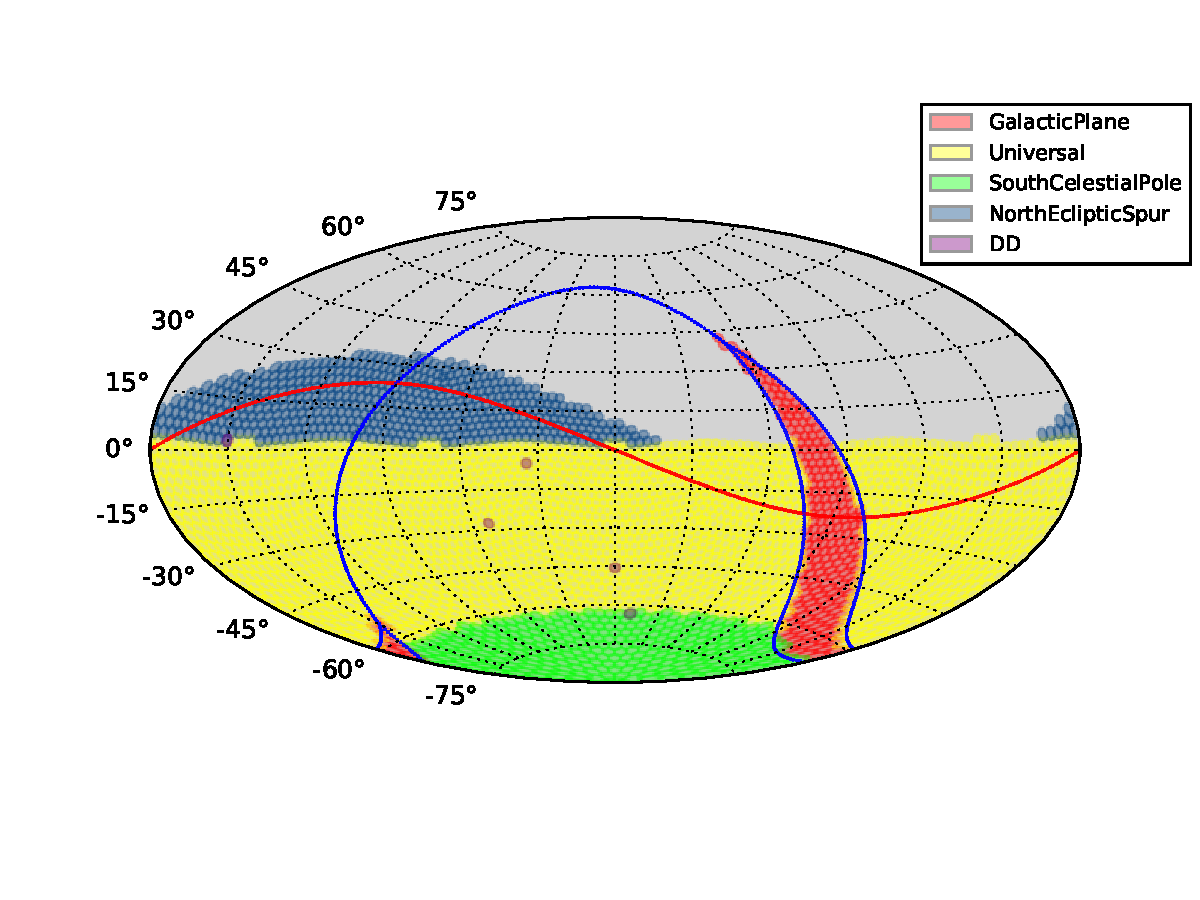
\includegraphics[width=.6\linewidth]{minion_1016_proposal_footprint.pdf}
\plotone{Figures/minion_1016_proposal_footprint.pdf}
\caption{Regions of the sky with different requirements and constraints for scheduling: (1) Galactic Plane Region (GP), (2) Universal or Wide Fast Deep (WFD), (3) South Celestial Pole (SCP), (4) North Ecliptic Spur (NES), and (5) Deep Drilling Fields (DD). This figure is taken from \citep{jones2017large}, with the author's permission.}
\end{center}
\end{figure}\label{fig_proposals}

The desirables and the constraints for different regions vary in both quantity and quality, see \citep{ivezic2008lsst} for a detailed explanation of the surveys associated with the sky regions. The notion of the features however, enables the scheduler to systematically fetch all of the various requirements and turn them into comparable quantities for the purpose of the decision making in the Markovian framework.

The feature-space of the LSST contains seven features (see Section~\ref{sec_lsst_features}), each can be evaluated given a field $i$, a filter $f$, and a time $t$. The fields are created to discretize the space through a fixed partitioning of the sky with ID numbers preassigned to them. Each field can be captured through a single visit, that lasts for 30 seconds. There are 6 possible filters, $[u,g,r,i,z,y]$ for a visit. And finally the time domain is discretized by the natural timing of the process. In other words, $t_j$ is exactly the moment that the $j$'th visit is over and the scheduler makes a decision for the next visit. Since a consecutive visit of the same field-filter is not allowed, there is a slew time between any two decisions, therefore $t_{j} - t_{j-1} > 0$. On the other hand, the operation is over a limited time horizon, $T$, thus the number of the decision time steps is finite. A finitely discretized sky, a finite number of the filters and a finite number of the time steps, define a finite feature-space, denoted by $\{(f_1(i,f,t_j)\dots f_7(i,f,t_j)): i = 1\dots n_f, f\in \{u,g,r,i,z,y\}, j = 0,\dots N\}$.

Then the implication of the policy, stated in Equation (\ref{equ_approx_pol}), for the LSST scheduler is as follows,

\begin{equation}\label{equ_approx_pol_imp}
\tilde{\pi}^*(x_j)= \argmin_{(i,f)\in \pazocal{A}_{j}} \sum_{k=1}^5 \theta^*_k E_{\pi}[\Phi_k(X_{j+1}) | x_j]\\,
\end{equation}
where $x_j = [f_{1, \dots,7}(id(t_j),ft(t_j),t_j)]$ is the 7-dimensional state at $t_j$, and $(i,f)$ is a feasible pair of field-filter. Section~\ref{sec_cstr} introduces the constraints under which a field-filter pair, $(i,f)$ is feasible at $t_{j}$. Accordingly, $\pazocal{A}_j$ is  the set of all field-filter pairs that are feasible at $t_j$.

In line with modular approach to the implementation of the scheduler, expected value of the basis functions, $E_{\pi}[\Phi_k(x_{j+1})|x_j]$ for $k=1,\dots, 5$ are evaluated in separated modules, developed by the LSST community. For instance, see \citep{sebag2008lsst} and \citep{sebag2007lsst}, for cloud cover measurements at the LSST site that were used to develop a cloud model and, see \citep{yoachim2016optical} for the sky brightness predictive model, specifically developed for the LSST. For the details of the basis functions of the Feature-Based scheduler for LSST refer to Section~\ref{sec_lsst_bfs}.

The last step is to implement the training procedures, (described in Section~\ref{sec_opt}) on the LSST model to derive $\theta^*$. Training of the LSST scheduler is explained in Section~\ref{sec_lsst_opt}, adopting two sample objective functions. However, the LSST community, and basically any individual can design their own mission objective function, whether it allows for well-defined instant rewards or not, then train the scheduler through the open source training code, and find a new set of $\theta^*$, that principly leads to a different behavior of the scheduler due to different objectives.


\subsection{Features of the LSST scheduler}\label{sec_lsst_features}

For designing the features, it is important to avoid redundancy and ensure the inclusion of determining information. It is also critical to hold a modular approach in the delivery of the information to the decision procedure. For instance, consider the amount of time, $\Delta t$, it takes for a telescope to move on from a visit, characterized by a pair of $(i_1,f_1)$, to the next visit $(i_2,f_2)$,  where, $i_1$ and $f_1$ are the current field and the current filter respectively, and $i_2$ and $f_2$ are the next field and the next filter respectively. In LSST problem, $\Delta t$ mainly depends on the slew time, mechanical settling time, the dome placement time (if a dome placement is required), and finally the time it takes to change the filter from $f_1$ to $f_2$. All of these timings are available through a precise simulation of the LSST model \citep{delgado2014lsst}. For all possible $(i_1,f_1)$, and $(i_2,f_2)$ a modular design would be to bring the summation of the operational timings to the stage of the decision, instead of bringing them separately as different features. This approach makes the implementation significantly simpler, more readable, and easier to debug, and in a conceptual level, makes it possible to track the effect of the operational timing in the overall outcome of the decision maker. Particularly, since the operational cost is independent of the amount to which each cause contributes to the overall $\Delta t$, bringing the timing of the separate procedures separately in the decision making level adds unnecessary complications to the design, and consequently, makes it hard to back track the output-input behavior of the scheduler. 

This section presents the features in Table (\ref{tab_features}), designed to efficiently carry the determining information with a modular approach. Each feature is denoted by $f_k(i,f,t)$ for $k= 1..7$, and indexed by the triplet of $(i,f,t)$, field, filter, and time. To make a decision at $t$, the scheduler computes all of the seven features for all of the $(i,f)$ pairs in general, however, there are some features that don't change in every time step, for instance, if $i$ is not visited at $t^j$, then $f_5(i,f,t^j)= f_5(i,f,t^{j+1})$. For such cases, the implementation has a categorized updating procedure to avoid extra computations.


\begin{table}[h]
\begin{tabularx}{\textwidth}{| l | X |}
\hline
Notation & Definition\textbackslash Description\\ \hline \hline 
$f_1(i,f,t)$ & ($slew(id(t),i)+settling(id(t),i)+\Delta t_{f} I_{ft(t) \neq f} \vee t_{dome}(i)$): either the time required to point the telescope to $i$, and change the filter to $f$, or the time required to relocate the dome to make $i$ visible. Whichever that is larger.\\ \hline
$f_2(i,f,t)$ &  the total number of the same-night visits of field-filter $(i,f)$ until $t$.\\ \hline
$f_3(i,f,t)$ &  $(t - \tau_n(i,f,t)) I_{\{\theta(i,f,t) > \tau_s(t)\}}$, time since the last same-night visit of $(f,i),$\\ \hline
$f_4(i,f,t)$ &  remaining time for field-filter $(i,f)$ to become invisible, either by passing the airmass or the moon-separation threshold, or being covered by temporary objects such as the clouds, as projected at $t$.\\ \hline
$f_5(i,f,t)$ &  co-added depth, a measure of cumulative quality of past visits of field-filter$(i,f)$ until $t$.\\ \hline
$f_6(i,f,t)$ &  $5\sigma$-depth, a measure for quality of visiting field-filter $(i,f)$ at $t$, depending on seeing, sky brightness, and airmass. $f_6(i,f,t) = C_m + 2.5 \log (\frac{0.7}{\sigma(i,t)}) + 0.50 (br(i,t)-21) - K(i,f) am(i,t)$ where $C_m$ is scaling coefficient.\\ \hline
$f_7(i,t)$  & hour angle of field $i$ at $t$.\\ \hline
\hline
\end{tabularx}
\end{table}\label{tab_features}

\subsection{Basis functions of the LSST scheduler}\label{sec_lsst_bfs}

Basis functions are fully determined by the value of the features, and are denoted by $\Phi_k(f_1(i,f,t),\dots, f_7(i,f,t))$, for $k = 1 \dots 5$. Each $\Phi_k$, is indexed by a triplet of $(i,f,t)$, time, field, filter, and is evaluated at every decision making step, $t_j$, for all field-filter pairs $(i,f)$. Similar to the update procedure of the features, for a decision at time $t_j$, all six basis functions would be evaluated for all pairs of $(i,f)$, except for the field-filters that are infeasible at $t_j$. Feasibility of a field-filter can be evaluated after the evaluation of the features, by applying the constraints of the region that the field belongs to (see Section~\ref{sec_cstr} for the list of constraints). Thus, while it is required to evaluate the features for all possible pairs of $(i,f)$ at all decision steps, the number of the basis functions to be evaluated is on average approximately a factor of three less than the number of the features.

The main strategy to incorporate the idea of features for the scheduling problem of the LSST is to define a  set of common basis functions and then modify them according to the requirements of each region. 


\subsubsection{Common basis functions}

Generally speaking, making a decision for a visit at $t$ for the LSST scheduling problem is mainly determined by the following factors,

\begin{enumerate}
\item The amount of the time it takes to redirect the telescope and the dome to move from one target to the next target,
\item The short-term science-driven requirements, such as the same-night revisit of a field within a valid time window in WFD, and NES surveys,
\item The long-term mission-driven requirements, such as maintaining a uniform coverage of all field-filter pairs within each region,
\item The relative quality of visiting a field-filter compared to other field-filters at the time of observation, for overall efficiency of the operation,
\item the general preference for observing the fields around the meridian.
\end{enumerate}

Accordingly, the basis functions of the LSST scheduler, are designed to formalize the above factors. Common basis functions that are shared amongst all of the regions, are defined in Table~\ref{tab_commonBF}.


\begin{table}[h]
\begin{tabularx}{\textwidth}{| l | X |}
\hline
Notation & Definition\textbackslash Description\\ \hline \hline
$\Phi_1(f_1(i,f,t))$ & $s_1.f_1(i,f,t)$, the cost of the required time for visiting field-filter $(i,f)$.\\ \hline
$\Phi_2(f_2(i,f,t))$ &$\begin{cases}0.5,& \text{if } \sum\limits_{f}{f_2(i,f,t)} = 0\\ 1,& \text{if } \sum\limits_{f}{f_2(i,f,t)} = 2\\ 0,  & \text{else,}\end{cases}$, \newline reflects the short term visit/revisit priority of field $i$, conditioned on the total number of the previous same-night visits.\\ \hline
$\Phi_3(f_5(i,t))$ &  $(1 - \frac{f_5(i,f,t)}{\max_\iota \max_\phi f_4(\iota,\phi,t)})$, reflects the long-term visit priority of field-filter $(i,f)$, based on the ratio of its co-added depth to the maximum co-added depth of all pairs of field-filter until $t$.\\ \hline
$\Phi_4(f_6(i,f,t))$ & $1 - Pr(f_6(\iota,\phi,t) \leq f_6(i,f,t))$, complimentary empirical CDF of $5\sigma$-depth of all $(i,f)$ pairs at $t$. $\Phi_4$ assigns a cost to field-filter $(i,f)$ based on its relative visiting quality compared to the other field-filter pairs at $t$.\\ \hline
$\Phi_5(f_6(i,f,t))$ &  $\frac{|hr(i,t)|}{12}$, encourages visiting of the fields near the meridian.\\ \hline
\end{tabularx}
\end{table}\label{tab_commonBF}

In the definition of $\Phi_1$ scale factor $s_1= 0.43$ is empirically evaluated to ensure that 80\% of the observed values of this basis function for the winner states are between 0 and 1. Scaling the values of basis functions is a regulation that in general results in a faster rate of convergence in the training process of the scheduler, and does not harm the optimality of the solution.

\subsubsection{Region-specific modifications of the common basis functions}

As mentioned in Section~\ref{sec_lsst_problem}, the LSST's mission poses different requirements on different regions of the sky. This section presents how we modified the common basis functions to accommodate different desirables of the Wide Fast Deep (WFD), North Ecliptic Spur (NES),Galactic Plane Region (GPR), and South Celestial Pole (SCP)  surveys. Deep Drilling Field (DDF) survey, however, contains a very small fraction of the visible sky's area, thus for the relatively rare event of the DDF observation, instead of modifying the policy we prescribe a schedule, and interrupt the operation of the scheduler. Particularly because, the recoverability attribute of the Feature-Based scheduler enables the scheme of the interruptions to be a part of the decision making procedure. In other words, if the interruptions are not too frequent, the Feature-based scheduler will recover itself back to the normal behavior, without requiring any information about before the interruption. 

\subsubsection{Controllability of the scheduler}\label{sec_sim_cont}

As discussed in Section~\ref{sec_SM}, the mission's objective has to be controllable via the design parameters, $\theta$. In this section we present an empirical measure of the mission's objective controllability. If the value of the objective function does not sufficiently respond to the variations of the design parameters, it is a sign of poor choice of the basis functions and/or input information. Either of these factors lead to a structure that does not admit a sufficiently optimal solution, and if on the other hand, the objective function is extremely variable with respect to the changes in the design parameters, the solution of the training is not reliable because the objective is not a well-behaved function of the optimization variables.

Fig~\ref{fig_controlability}, shows a few one dimensional slices of the following simple objective function (\ref{equ_short_term_U}), evaluated after about five hours of scheduling , with different $\theta$'s in $[0,10]$ range. To measure the variability of the objective function with changes in the $i$'th basis function, we define a sequence of equidistant values for $\theta_i \in \{\theta_i^{j_1},\dots,\theta_i^{j_m}\}$ and keep the other $\theta$'s fixed, then run the scheduler for $T = 4.8 hrs$ with all resulting $\theta$'s that are different by the $i$'th element, then evaluate $U_{\pi_{\theta}}(.)$, defined as follows, to be a (simple) mission objective that reflects the slew time $slew(.)$ and airmass $am(.)$ aversion,

\begin{equation}\label{equ_short_term_U}
U_{\pi_{\theta}}(x_0,x_{1}, \dots, x_{n})= -\sum_{\{i:t_0<t^i<t_n\}} {slew(id(t_{i}), id(t_i)) + 10 . am(id(t_i))}
\end{equation}

\begin{figure}[h!]
\begin{center}
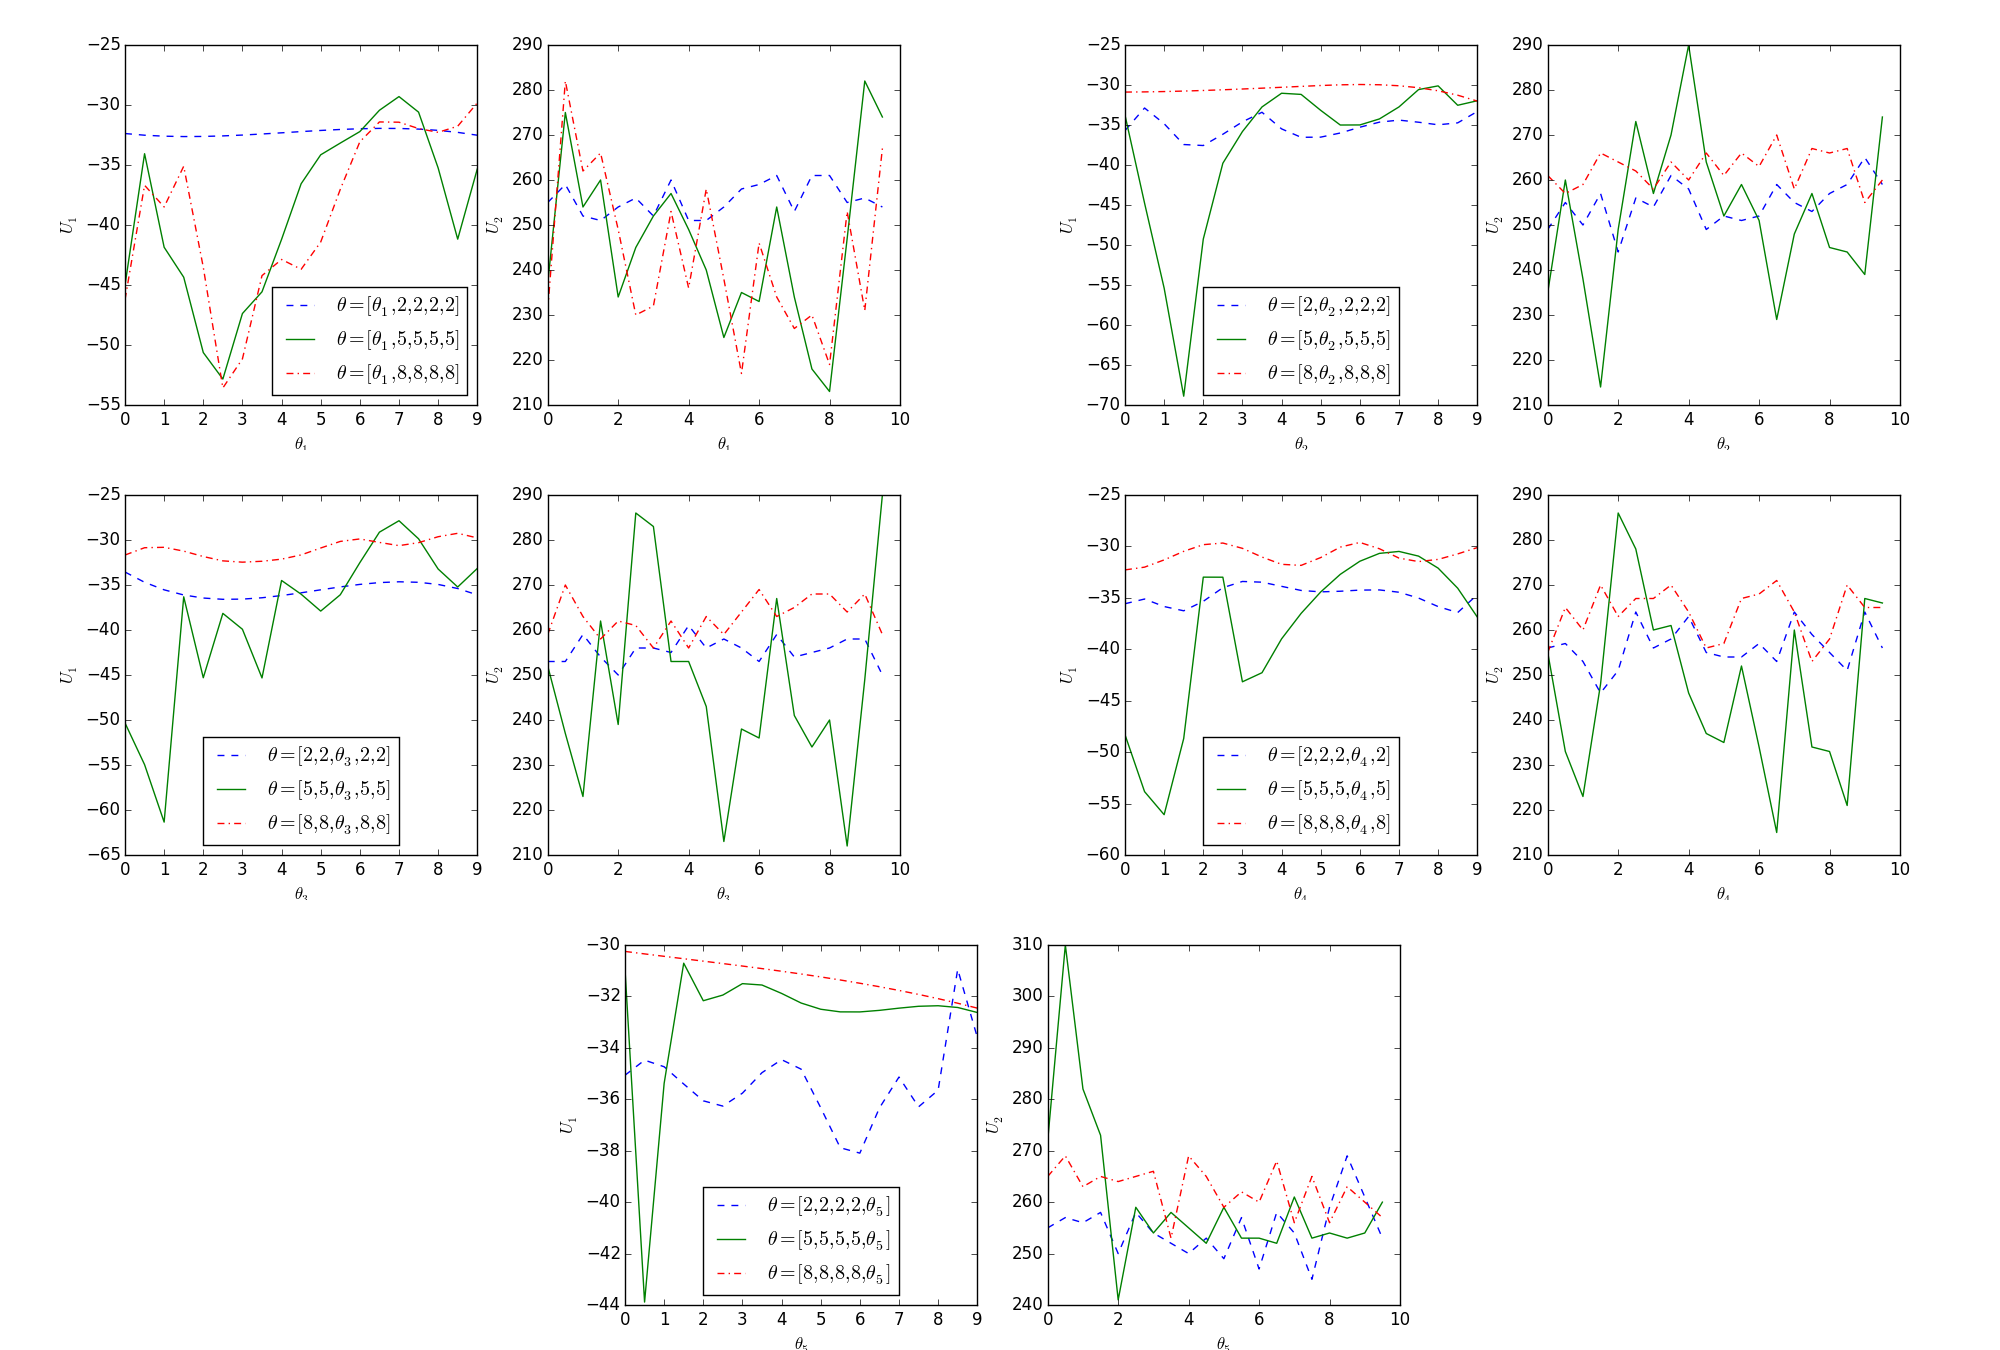
\includegraphics[width=1\linewidth]{Figures/Controlability.png}
\end{center}
\caption{Slices of the Objective function (\ref{equ_short_term_U}). The variation of the objective function, specially in the mid-range slices (solid line) demonstrates the controllability of the scheduler's performance with the design parameters.}
\label{fig_controlability}
\end{figure}

Figure~\ref{fig_controlability}, contains slices of the 5-dimensional $U_{\theta }(t_0, T)$, and the total number of visits between $t_0$ and $T$. Both of the simple objective function and the total number of visits reasonably respond to the changes in all five dimensions of the variable $\theta$, which demonstrate the controllability of the objective function. Moreover, the smaller variations for slices closer to the boundaries of the search space, suggest that the design and scaling of the basis functions provides a desirable behavior for the objective function within the proposed search space.


\begin{table}[h!]\label{tab_regionBF}
\begin{tabularx}{\textwidth}{| X | X |}
\hline
Modified basis functions & Description\\ \hline \hline

$\begin{array}{l c l}\Phi_1^{\text{WFD}}(f_1) &=& \Phi_1(f1)\\ \Phi_1^{\text{NES}}(f_1) &=&\Phi_1(f_1)\\ \Phi_1^{\text{GPR}}(f_1) &=& \Phi_1(f_1)\\\Phi_1^{\text{SCP}}(f_1) &=&\Phi_1(f_1)\end{array}$  

& No modification is required, because the cost associated to the timing of the operation is independent of the survey.\\ \hline

$\Phi_2^{\text{WFD}}(f_2,f_3,f_4) =$ \newline $\begin{cases} \Phi^{\text{pair}}(f_3)I_{f_4> W_2},& \text{if } \sum\limits_{f}{f_2} = 1,\\ \Phi_2(f_2),& \text{else } \end{cases}$ \newline\newline $\Phi_2^{\text{NES}}(f_2,f_3,f_4) =\Phi_2^{\text{WFD}}(f_2,f_3,f_4)$ \newline\newline $\Phi_2^{\text{GPR}}(f_2) = \Phi_2(f2)$ \newline\newline $\Phi_2^{\text{SCP}}(f_2) = \Phi_2(f2)$\newline\newline $\Phi^{\text{pair}}(f_3) :=$ \newline $\begin{cases} \exp(- \frac{\min_{\phi}f_3(i,\phi,t)}{W_2})& \min_{\phi}f_3(i,\phi,t) < \frac{W_2}{2}\\ 0, & \text{else}\end{cases}$ 

& The WFD and NES surveys require pairs of visits for which a second same-night visit has to be scheduled in a certain time window, $[W_1,W_2]$. $ \Phi^{\text{pair}}$ is defined to encourage second valid visits. There is no revisit strategy for GPR and SCP fields because they receive at most one visit per night in the baseline LSST mission, hence no modification is required.\\ \hline


$\begin{array}{l c l}\Phi_3^{\text{WFD}}(f_5) &=& s_{WFD} \Phi_3(f_5)\\ \Phi_3^{\text{NES}}(f_5) &=& s_{NES} \Phi_3(f_5)\\ \Phi_3^{\text{GPR}}(f_5) &=& s_{GPR} \Phi_3(f_5)\\\Phi_3^{\text{SCP}}(f_5) &=& s_{SCP} \Phi_3(f_5)\end{array}$ 

& The total number of the required visits is different for fields in different surveys, to take this difference into account, we set $s_{WFD} = 1$, and scale the third basis function of other regions according to the ratio of the required visits with respect to the required visits of the WFD survey.\\ \hline

$\begin{array}{l c l}\Phi_4^{\text{WFD}}(f_6) &=& \Phi_4(f6)\\ \Phi_4^{\text{NES}}(f_6) &=&\Phi_4(f_6)\\ \Phi_4^{\text{GPR}}(f_6) &=& \Phi_4(f_6)\\\Phi_4^{\text{SCP}}(f_6) &=&\Phi_4(f_6)\end{array}$  

& $\Phi_4$ is defined to account for the observing quality of each field-filter compared to the others, which is independent of the survey that the field belongs to, therefore no region dependent modification is required.\\ \hline
 
$\begin{array}{l c l}\Phi_5^{\text{WFD}}(f_7) &=& \Phi_5(f7)\\ \Phi_5^{\text{NES}}(f_7) &=&\Phi_5(f_7)\\ \Phi_5^{\text{GPR}}(f_7) &=& \Phi_5(f_7)\\\Phi_5^{\text{SCP}}(f_7) &=&\Phi_5(f_7)\end{array}$  
& near meridian observation is equally desirable for all of the regions, therefore no modification is required. \\ \hline

\end{tabularx}
\end{table}


\subsection{Survey-specific constraints}\label{sec_cstr}

The scheduler's decision at each time step is an admissible pair of field-filter $(i,f)$, an the feasibility of a candidate pair is driven by the following factors:

\begin{itemize}
\item Visibility: The candidate field-filter has to be visible.
\item Quality: The expected observational quality of a field-filter has to be beyond the given lower threshold.
\item Survey's timing: The science-Driven revisit constraints has to be respected.
\end{itemize}

Exact expression of the LSST scheduler constraints are presented in Table~\ref{tab_feasibility}.

\begin{table}[h!]
\begin{tabularx}{\textwidth}{| l | X | X | l |}
\hline
& Feasibility of field-filter $(i,f)$ for a visit at $t^{n+1}$, as evaluated at $t^n$& Description & region\\ \hline \hline

1&$ \tau_{rise}(i,f,t^{n+1}) \leq t^{n+1} \leq \tau_{set}(i,f,t^{n+1}) $ & field-filter $(i,f)$ has to be above the acceptable airmass horizon at $t^{n+1}.$ & All regions\\ \hline

2&$ E[f_4(i,f,t^{n+1})] \neq 0 $ & field-filter $(i,f)$ is not temporarily masked at $t^{n+1}$. & All regions\\ \hline

3 & $\sum_{f}f_2(i,f,t^n) < N^{\textit{survey}}$ & $N^{\textit{survey}}$ poses a region dependent upper-bound on the number of the visits for each field. $N^{WFD}= N^{NES} = 3$, and $N^{GPR}= N^{SCP} = 1.$ & All regions\\ \hline

4 & $E[f_6(i,f,t^{n+1})] < \sigma({\textit{survey},f})$ & the expected quality of visiting field-filter $(i,f)$ at $t^{n+1}$ has to be better than the given threshold, $\sigma(.)$, that depends on the survey and the filter. & All regions\\ \hline

5&$f \neq id(t^n)$ & consecutive visit of a same field is not allowed. & All regions\\ \hline

6& if $\sum_{f}f_2(i,f,t^n) = 0$ then \newline $\max_\phi f_4(i,\phi,t^n) > \frac{W_1+W_2}{2}$ & the first visit of field $f$ has to occur $\frac{W_1+W_2}{2}$ time before it becomes invisible, so that the second visit of $f$ can be scheduled in the valid time window. & WFD and NES\\ \hline

7& if $\max_{\phi}\theta(i,\phi,t^n) > \tau_s(t^n)$ then \newline $ W_1 \leq \min_{\phi}f_2(i,\phi,t^n) \leq W_2 $& if there has been a same-night visit of field $f$ until $t^n$, then the next same-night visit has to occur in the valid time window. & WFD and NES\\ \hline

8&if \newline $\max_{\phi}\theta(i,\phi,t^n) > \tau_s(t^n)$ then \newline $f \notin \{\text{y},\text{u}\}$& if there is a same-night visit of field $f$ until $t^n$, then the next same-night visit cannot be with either of u or y filters. & WFD\\ \hline

9& $f \notin \{\text{y},\text{u}\}$ & visits with u filter and y filter is not allowed. & NES\\ \hline

\end{tabularx}
\end{table}\label{tab_feasibility}


\section{LSST scheduler optimization}\label{sec_lsst_opt}

For both of the reinforcement learning and the global optimization approaches, discussed in Section~\ref{sec_opt} we used a simulated model of the telescope and the environment, including the brightness model of the sky and coverage of the clouds, developed based on the measurements at the LSST site. 


\subsection{LSST scheduler reinforcement training}

The simulation for the reinforcement learning starts at $t_0 = 2462867.5~mjd$ (January 1, 2021), with $\theta^0 = (10,10,10,10,10)$, initialized to give the non-negative variables enough space to decrease , and continues until $\theta$ converges. Figure~\ref{fig_theta_conv}, is the training curve for all of the variables over a course of 3000 decisions, for the following instant reward. The discount rate of $\gamma = 0.9$, and learning rate of $\frac{0.01}{\log^3(i)}$ are chosen empirically. 

\begin{equation}
r(s_{i-1}, s_i) = -slew(id(t_{i-1}), id(t_{i})) - am(id(t_i))
\end{equation}

\begin{figure}[h!]
\begin{center}
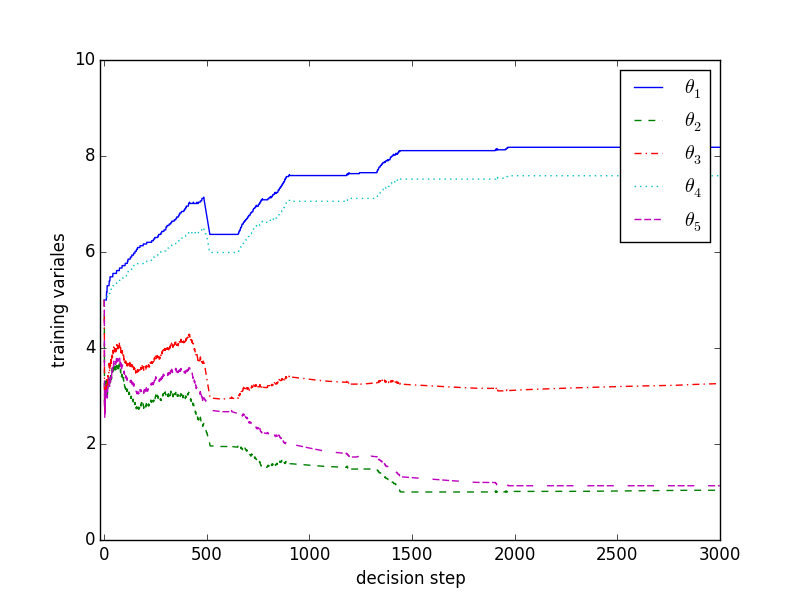
\includegraphics[width=0.4\linewidth]{Figures/TDcurve.png}
\end{center}
\caption{}
\label{fig_theta_conv}
\end{figure}

For the above choice of reward, $\theta$ converges to the following solution:

\begin{equation*}
\theta^* = (8.18,  1.04,  3.26,  7.59,  1.13).
\end{equation*}

In this approach, the computational time to evaluate the update is negligible with respect to the time required to evaluate the features, therefore, the computational time of the reinforcement learning is almost equal to the simulation of the scheduling (without any updates) which is linear with respect to the number of the decisions. With a personal computer \footnote{Processor: 1.6 GHz, Memory: 4 GB 1600 MHz DDR3}, each decision takes about $0.5$ second, thus the time of the convergence for the simulation, presented in this session is $3000\times 0.8 \text{ sec } = 40 \text{ minutes }$.

\subsection{LSST scheduler global optimization}

One of the important simple objective functions that cannot be expressed as the discounted sum of the rewards is the total number of the observations in an episode of the simulated operation from $t_i$ to $t_j$,

\begin{equation}\label{equ_lsst_ede}
U_{\pi_{\theta}}(x_i, x_{i+1}, \dots, x_j) = j - i.
\end{equation}

The following regulatory constraints are applied to $\theta$ for the global optimization approach:

\begin{itemize}
\item $\theta \geq 0$: The basis functions, $\Phi_i(.), i = 1\dots 5$, are designed to reflect the operational cost, therefore a linear combination with positive coefficients $\Phi(s_{t^n})= \sum_{i=1}^5 \theta_i \Phi_i$, would reflect the cost of the operation that we minimize in our policy.

\item $\theta_1 =\theta_0$: We pick a constant value for the first element of $\theta$ to reduce the dimension of the optimization problem by one. This is possible without the loss of generality because each element of $\theta$ does not have a meaningful inherent value, and in fact, its value compared to the other elements determines the behavior of the policy. In other words, if $\theta^*$ yields an optimal scheduler, then $\alpha \theta^*$ for $\alpha > 0$ yields and optimal scheduler due to the design of the policy (\ref{equ_approx_pol}), where, 

\begin{equation*}
\argmin_{a_{i}} \sum_{j=1}^k \theta^*_j E[\Phi_j(X_{i+1}) | a_{i}] = \argmin_{a_{i}} \sum_{j=1}^k \alpha \theta^*_j E[\Phi_j(X_{i+1}) | a_{i}].
\end{equation*}
\end{itemize}


We used the above objective function (\ref{equ_lsst_ede}) for $t_i = 2462867.5~mjd$ (January 1, 2021) and $t_j = 2462877.5~mjd$ (January 11, 2021). Figure~\ref{fig_eDEObjectiveFunction}, shows the value of the objective function over the iterations of the $e$DE algorithm. The following $\theta$ yields the best $U_{\pi_{\theta}}$ after 50 iterations for $\theta_1 = 1.00$, and $\theta_U = 10.00$:

\begin{equation}
\theta^* = (1.00, 0.84, 0.99,  1.34  3.04).
\end{equation}



\begin{figure}[h!]
\begin{center}
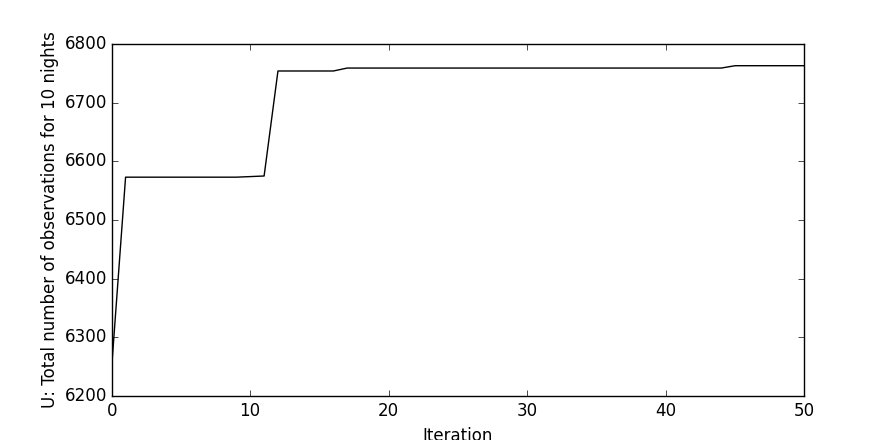
\includegraphics[width=0.5\linewidth]{Figures/eDEObjectiveFunction.png}
\caption{Progress of the objective function (\ref{equ_lsst_ede})} over the iterations of the $e$DE algorithm.
\label{fig_eDEObjectiveFunction}
\end{center}
\end{figure}

$e$DE is a population-based metaheuristic algorithm, and for the result shown in Figure~\ref{fig_eDEObjectiveFunction}, number of the population $N_P$ is set to be 50. Each function evaluation is in fact, the simulation of 10 days of scheduling with a candidate scheduler which takes about 8 minutes, therefore each iteration, in total, takes $N_P * 8$ minutes with a personal computer\footnote{Processor: 1.6 GHz, Memory: 4 GB 1600 MHz DDR3}. The optimization can be manually terminated if the result is satisfactory, or can be continued until a full convergence. In $e$DE (and all genetic algorithms in general), function evaluation for each individual is independent from other individuals, therefore the parallel implementation of the same algorithm can be faster up to a factor of $N_p$. 

 


\section{Performance of a Modified Feature-Based scheduler for LSST}\label{sec_comp}

In this section, the LSST Metric Analysis Framework \citep{jones2014lsst} is used, to compare the performance of an modified version of the Feature-Based scheduler with \textit{astro-lsst-01-2013}, the most recent official schedule of the LSST, over a 10 year period of simulations, starting from January 1, 2021.  The LSST scheduler is under active development, and can be found at \url{https://github.com/lsst/sims_featureScheduler}.


In \S\ref{sec_lsst_opt}, we showed we can optimize a Feature-Based scheduler, and now we modify the scheduler presented above to address some observational details with LSST.  Note that rather than tracking potential pointings as distinct field-filter pairs, we track the progress of the survey with high resolution HEALpixel maps. The mapping of HEALpixels to final discrete pointing can then be randomized each night, spatially dithering the resulting observations. For the Modified Feature-Based scheduler, we use five basis functions:
\begin{enumerate}
\item{A HEALpix map that tracks how many observations have been taken across the sky and compares it to an ideal coverage map.}
\item{A map of the current 5$\sigma$ limiting depth minus the 5$\sigma$ depth map of when a point is on the meridian in dark time. This effectively combines throughput considerations based on the current sky brightness, airmass, and filter choice.}
\item{A map showing how much time it would take to slew to given positions in the sky.}
\item{A mask which limits where the telescope can slew in altitude and azimuth, including mechanical exclusion areas and exclusion areas around the moon and bright planets.}
\item{A penalty for changing filters. This penalty is lifted when twilight starts or stops and when the moon rises or sets.}
\end{enumerate}
These basis functions are used to compute a reward function for each filter, and the observation with the highest reward is selected. In addition to the six filters, there is a separate process tracking if an observation will need to be observed in a pair, and separate processes deciding if a deep drilling sequence should be executed. Because the mask basis function is binary, there are only four free parameters that control the behavior of the modified Feature-Based scheduler. 

The modified Feature-Based scheduler is being developed to address the specifications of the LSST's scheduling. Improvements are mainly on the definitions of the basis functions and the constraints without breaking the memorylessness (they still, only depend on the current state),  linearity, and modularity of the design, therefore the parameters can be optimized or trained by the proposed algorithms. Here we present a manually adjusted version of the modified Feature-Based scheduler, and show that even without automated training, it outperforms the best outcome of the current official LSST's scheduler, \textit{astro-lsst-01-2013}, a heavily tailored scheduler by human experts. 

For a survey telescope, co-added depth, as a measure of the cumulative information collected from each direction of the sky, has to be ideally uniform within each of the five regions. Figure~\ref{fig_10yrs_skymap} demonstrates the final value of the co-added depth after 10 years of scheduling simulation in all 6 filters, for both modified feature-based algorithm and \textit{astro-lsst-01-2013}. Figure~\ref{fig_10yrs_hist} compares the distribution of the co-added depth on the (finely discretized) sky, and the fact that in all filters the distribution is more concentrated for feature-based scheduler, shows that the outcome is closer to the ideal of uniform coverage for the LSST mission, that would have a zero variance within each region.


\begin{figure}[h!]
\plottwo{Figures/OpSim10yrs_skymap.png}{Figures/FB10yrs_skymap.png}
\caption{The final co-added depth distribution in all six filters. According to the mission's objective, the scheduler has to provide a uniform coverage of the visible sky within each region, and in each filter. The left panels show the OpSim \textit{astro-lsst-01-2013} simulation results while the modified Feature-Based scheduler is on the right. We have closely matched the footprint of the original OpSim survey, as well as matched the regions that should be de-emphasized (such as the galactic plane and South celestial pole).  XXX--I think the FB wasn't respecting the cloud closure times, so some of the extra depth is a cheat. Need to mention that it's not a straight apples-to-apples comparison. But it might be nice to add zoom in plots (maybe near the WFD GP border) to show how the dithering smooths things out.}
\label{fig_10yrs_skymap}
\end{figure}


\begin{figure}[h!]
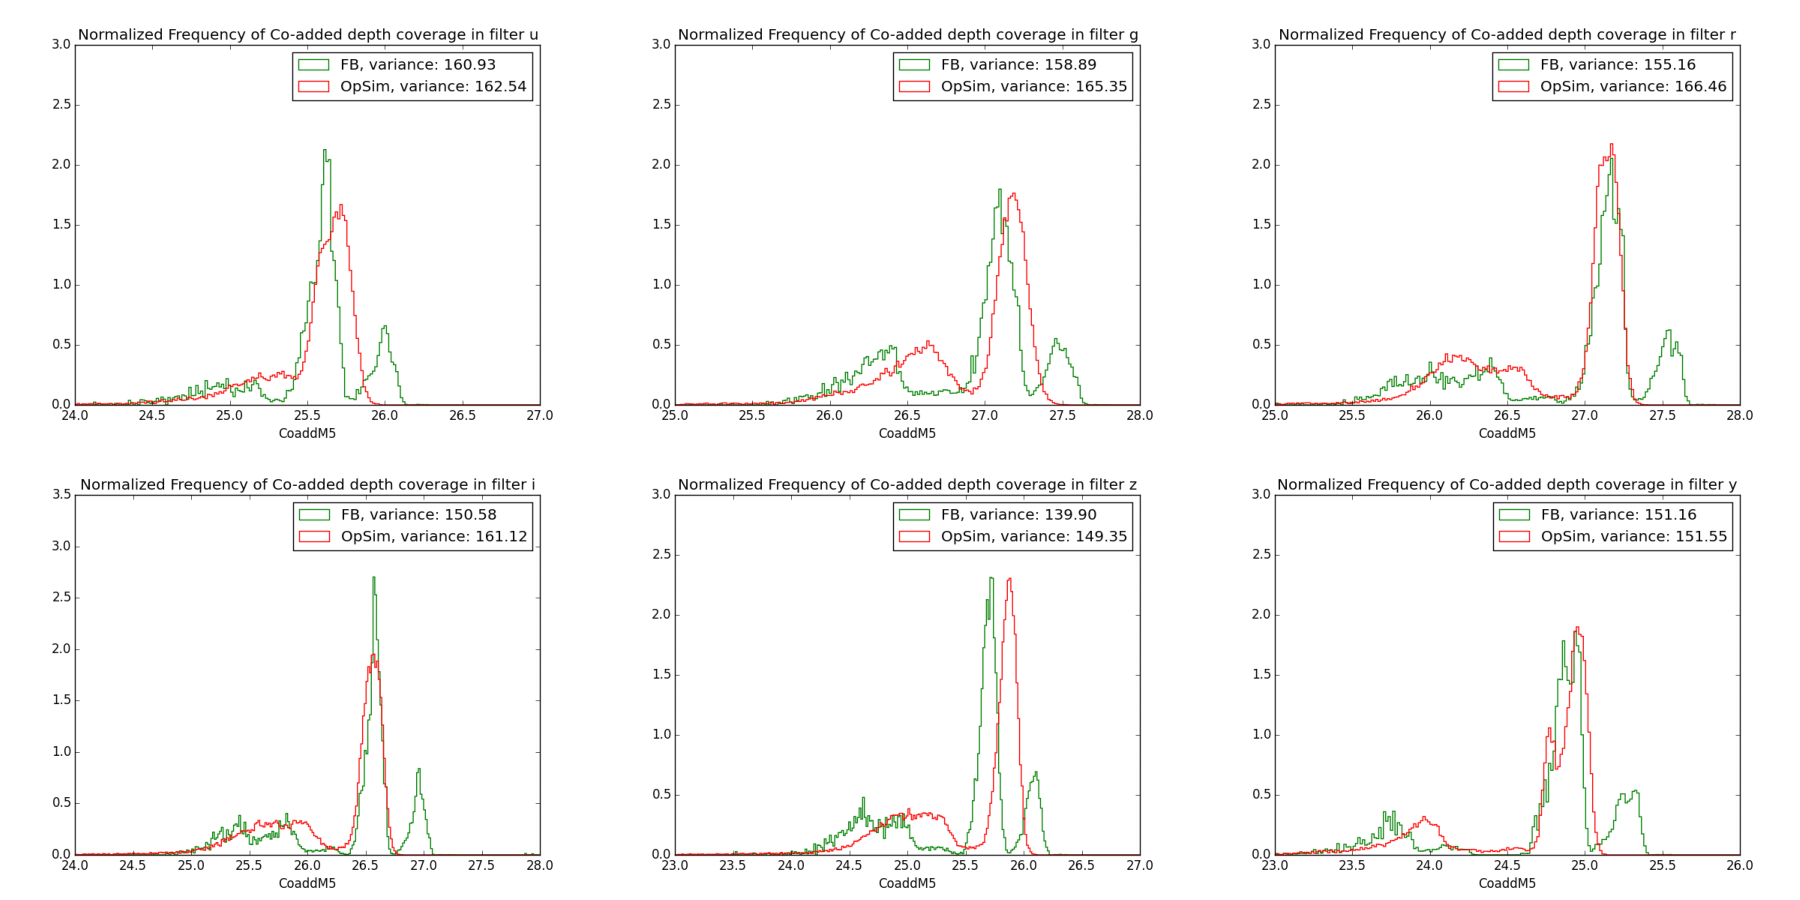
\includegraphics[width=.9\linewidth]{Figures/Co_addedHist10yrs.png}
\caption{Each plot compares the histogram of the final co-added depth in one of the six filters. LSST's mission calls for uniform coverage of the sky and prefers a smaller variance in the distribution of the the final co-added depth. Feature-Based scheduler offers a similar or sharper distribution of the the co-added depth after 10 years of the simulation in all filters. XXX--good place to point out this is the dithering scheme in FB. OpSim has a small section of very deep observations due to field overlaps. By dithering, FB is able to move the peak deeper. That's why I'm 99\% sure the green line should be labeled as from OpSim.}
\label{fig_10yrs_hist}
\end{figure}


In addition to uniformity of the coverage, the LSST mission calls for pairs of the visits within a valid window at the same night. The main reason is to be able to detect the transient objects such as asteroids. Since, the moving objects usually belong to the solar system, the pair constraint was initially imposed only on the WFD and NES regions. However, there are interesting solar system objects such as interstellar asteroids that can be observed in any direction of the sky, therefore we made the pair constraint a universal constraint for all of the regions, besides other varying objects, such as super novae, can enjoy a follow up visit for the classification purposes, specially if the second visit is with a different filter than the earlier visit. The downside of this extension is that it constrains the scheduler even more and the performance can be potentially less than it could be. Note that the structure of the Feature-Based scheduler, allows for extension or restriction of the constraints to the individual field's level, with neither contradicting any of the Markovian framework assumptions, nor breaking the structure of the implementation. Figure~\ref{fig_10yrs_pair} demonstrates the distribution of the observations in pair (in the $g$, $r$, and $i$ filters) to the total number of the observations. For the regions that the pair constraint is applied, this ratio can be interpreted as the success rate of the scheduler to satisfy the pair constraint. Figure~\ref{fig_10yrs_pair_hist}, compares the distribution of the visits-in-pair ratio of the modified Feature-Based scheduler and \textit{astro-lsst-01-2013}. Note that the peak of the density for Figure~\ref{fig_10yrs_pair_hist} is closer to $1$, which means a larger area of the sky is covered by successful visits-in-pairs, however, the Feature-Based scheduler offers a sharper concentration of the values that can be interpreted as higher uniformity of the visits-in-pair distribution, over the visible sky. In other words, the Feature-Based scheduler, sacrifices perfect visit-in-pair for a limited area of the visible sky to maintain a uniform ratio of visit-in-pair for a larger area of the sky.

\begin{figure}[h!]
\plottwo{Figures/OpSim10yrs_Pair_skymap.pdf}{Figures/FB10yrs_Pair_skymap.pdf}
\caption{The ratio of the visit-in-pairs (in the $g$, $r$, and $i$ filters) to the total number of the observations on the sky map. For the areas that the pair constraint is applied, the ratio is desired to be one. For feature-Based Scheduler, the pair constraint is applied to all of the regions and for \textit{astro-lsst-01-2013}, it is applied to the WFD and NES regions only.}
\label{fig_10yrs_pair}
\end{figure}


\begin{figure}[h!]
\centering
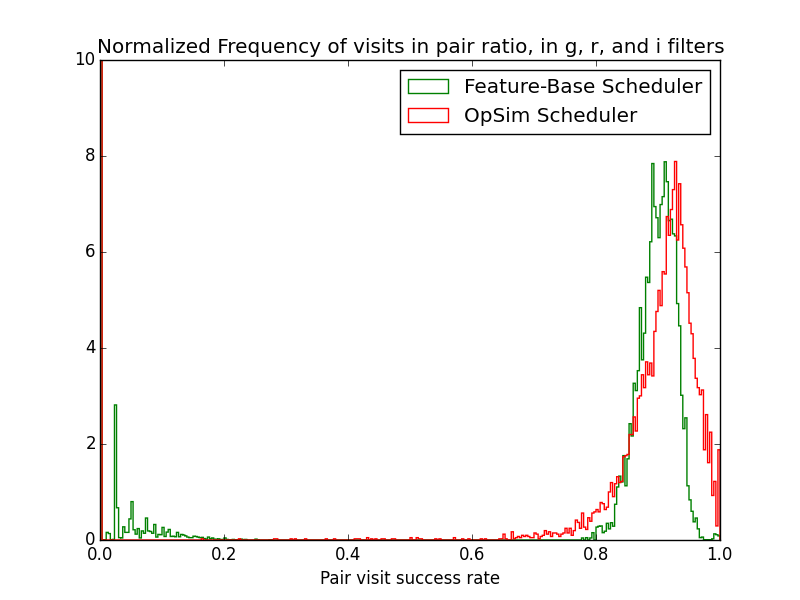
\includegraphics[width=.5\linewidth]{Figures/PairHist.png}
\caption{The Feature-Based scheduler in compare with \textit{astro-lsst-01-2013}, sacrifices perfect visit-in-pair for a limited area of the visible sky (with a lower mean) to maintain a uniform ratio of visit-in-pair for a larger area of the sky (with a sharper distribution)}
\label{fig_10yrs_pair_hist}
\end{figure}

Airmass is one of the major obstacles for high-quality observation. Although zenith observations have the minimum airmass, off-zenith observations cannot be avoided, because, not all of the celestial sphere passes through zenith, for which the best observation condition is when they are on the meridian. Therefore, observations around the meridian provide high quality data and consequently more efficient operation of the telescope. Figure~\ref{fig_10yrs_AltAz} compares the number density of the visits in altitude-azimuth map in each of the six filters $[u,g,r,i,z,y]$. Clearly in all filters, the modified Feature-Based scheduler schedules more visits around the desirable meridian zone. In addition, it offers a consistent concentration peak on the east wings, which is essential for a higher success rate for the visit-in-pair constraint. Because, if the first visit of the night occurs when the field is on the east side of the sky, it provides a longer time opportunity for the second visit of the same night. Note that flexibility of the Feature-Based scheduler allows for a significant change in the behavior, in this case a variant of the marching army cadence is incorporated to control the location of the visits through a basis function modification.

In Figure~\ref{fig_all_alt_az} and Table~\ref{OSF_table} we compare the modified Feature-Based scheduler with the previous LSST simulations \textit{astro-lsst-01-2013} and \textit{minion\_1016}. Ideally, we would compare the final depth of each simulated survey to judge their performance. Unfortunately, the simulations have been run with different sky background models and different weather downtime values, making a direct depth comparison impossible. We can make an approximate comparison by combining the surveys' open shutter fraction (OSF), median airmass, and if observations are dithered. The open shutter fraction is the total time the telescope camera shutter was open divided by the total time it could have been open. This reveals how well a scheduler is minimizing slew times and filter changes.  The median airmass measures how intelligently the scheduler is pointing the telescope, as lower airmasses have higher throughput. Finally, the default sky tessellation adopted by LSST includes significant overlap between fields, resulting in 23\% of the sky being covered by more than one field. By dithering the pointings, the median number of observations at a typical point in the sky increases by $\sim15$\%. Dithering is also essential for removing systematic effects for science cases such as measuring galaxy counts \citep{Awan2016}. In Table~\ref{OSF_table}, we compare our modified Feature-Based scheduler to two proposal based surveys produced by the LSST collaboration. The table shows that there is a tension between airmass and slewtime. The \textit{minion\_1016} gives high weight to minimizing slewtime, thus has the best OSF, but takes observations at the higher airmass. Meanwhile \textit{astro-lsst-01\_2013} gives a high weight to observing at low airmass, resulting in a lower OSF. In the $r$\ filter where atmospheric extinction is less relevant, \textit{minion\_1016} has a higher total throughput while \textit{astro-lsst-01\_2013} has higher throughput in the $g$\ filter. By including dithering, the modified Feature-Based scheduler vastly outperforms the other surveys in both the blue and red filters. The modified Feature-Based simulation has the lowest OSF, but this is an initial simulation where the basis function weights have not been optimized, so there is potential for improvement. Using the modified Feature-Based to schedule observations in large blocks could improve the OSF as shown in D. Rothchild et al. (2018, in preparation).


\begin{deluxetable}{lccccc}\label{OSF_table}
\tablecaption{Comparison of three different survey algorithms in a section of the LSST Wide-Fast-Deep survey area.}
\tablehead{
\colhead{Survey} & \colhead{OSF} & \colhead{median Airmass} & \colhead{dithered} & \colhead{median throughput}\\
  & &&& \colhead{$r$ (\%)} & \colhead{$g$ (\%)}
  }
\startdata
Modified F-B & 0.705 & 1.1 & yes & 63.7 & 47.0 \\
minion\_1016 & 0.736 & 1.2 & no & 55.3 & 40.0 \\
astro-lsst-01\_2013 & 0.715 & 1.1 & no & 54.4 & 40.8 \\
\enddata
\end{deluxetable}



\begin{figure}[h!]
\plottwo{Figures/OpSim10yrs_AltAz.png}{Figures/FB10yrs_AltAz.png}
\caption{Each plot is the distribution of the co-added depth on an altitude-azimuth map in one of the six filters for 10 years of the simulation. The higher concentration on the meridian (vertical axis) shows a more desirable behavior, because visits closer to the meridian are more efficient in terms of the quality of the visit compare to visits farther from the meridian with the same exposure time.}
\label{fig_10yrs_AltAz}
\end{figure}


% Figures generated by https://github.com/yoachim/18_scratch/blob/master/bosf_values/BOSF_check.ipynb
\begin{figure}
\epsscale{0.35}
\plotone{Figures/minion_1016_Observation_Density_HEAL_SkyMap.pdf}
\plotone{Figures/astro-lsst-01_2013_Observation_Density_HEAL_SkyMap.pdf}
\plotone{Figures/FB_Observation_Density_HEAL_SkyMap.pdf}
\epsscale{1}
\caption{The altitude azimuth pointing distribution for three LSST simulations. On the left, the proposal based minion\_1016 simulation takes most observations at high airmass and very few on the meridian. In the middle, the astro-lsst-01\_2013 simulation takes many observations on the meridian, but still executes deep drilling fields and a smattering of other observations at high airmass. On the right, the feature based simulation concentrates observations, including deep drilling fields, while avoiding observing near zenith. }\label{fig_all_alt_az}
\end{figure}

\section{Concluding remarks}\label{sec_conclusion}

This study demonstrated that a Markovian scheduler based on expert-designed features, and a parametrized decision making policy, can be successfully applied to multi-mission, ground-based telescopes. Unlike the mainstream telescope schedulers, Feature-Based scheduler does not require hand-crafted observation proposals and consequently improves the efficiency of the telescope's operation by bringing the decision making process to the individual observations level that are made for optimality as well as feasibility. Moreover, being modeled as a Markovian Decision Process, Feature-Based scheduler offers a systematic approach to the optimization of the scheduler's behavior under uncertainties. Schedulers that rely on human interaction are fundamentally prone to potential suboptimality, mainly because they are tailored based on inspections of the instances. Moreover, adjusting their behavior is inconvenient and time consuming in practice. 


On the other hand, the decision criteria in the Feature-Based scheduler are designed, and separated in an intuitive way for the astronomy community that allows for expert intervention if needed, however in a regulated way, and only on the parameters of the policy. Manual adjustments of the parameters of the policy does not break measurability, linearity, and memorylessness of the process. Thus all of the simplicity, optimality conditions and modularity of the design remain valid. In addition, due to the coherent structure, from training to online decision-making, Feature-Based scheduler is easy to understand, implement, and troubleshoot. Simplicity of the design and implementation, also provides a desirable environment for a wide-range of programming expertise in astronomy community to install the python packages on a local computer, define a custom mission objective, train a scheduler and examine the behavior of the scheduler with various objectives. Similarly, for a change in the mission's objective deriving a new scheduler that optimizes the new objective is principally automated. Furthermore, for the mission planning of the future telescopes a scheduler with adjustable objective can be extremely helpful, because it can answer high-level trade-off questions such as the amount of the time efficiency loss in different strategies of capturing transient objects. 

Furthermore, the required computational resource for the training/optimizing of the Feature-Based scheduler is versatile, depending on the purpose. If many different objective functions are being tested for planning a mission, then a quick $e$DE optimization for a short episode can find a sufficiently good scheduler for each mission or even a quick manual hand tuning to incorporate the intuitive importance of each basis function is possible because they carry an astronomical observation meaning. On the other hand if the objective is known and fixed, and the scheduler is being trained for real-time decision making, then one might even categorize the observation nights based on their main differences, such as the moon-phase and train a scheduler specifically for each category. 


\acknowledgments
XXX-Thanks everybody! (XXX-This is generally where who's supported by what goes)

\facility{LSST}

\software{MAF \citep{jones2014lsst}, healpy \citep{Healpy05}, matplotlib \citep{matplotlib07}, 
          astropy \citep{astropy18}, XXX-numpy/scipy}

%\bibliographystyle{unsrt}
%\bibliography{/Users/elahesadatnaghib/Dropbox/Graduate/Research/Princeton/Publications/references}
\bibliography{references}
\end{document}


